\chapter{System Design and Architecture for Intelligent Fault Detection and Predictive Governance}

Designing an intelligent fault detection system for power transmission lines requires careful consideration of real-time constraints, system scalability, and decision-making capabilities. The system must process high-frequency sensor data, accurately classify faults, and provide meaningful insights for operators. This chapter presents the design specifications, modeling choices, and architecture of the proposed multi-layered system. It also details the methodology and design considerations involved in integrating embedded machine learning, decision intelligence, and generative AI.

\section{Specifications for the Design}

The system is designed with the following specifications:
\begin{itemize}
\item Input: Real-time voltage and current sensor data from transmission lines
\item Output: Fault classification, risk score, and AI-generated insights
\item Model: Decision Tree for embedded real-time inference
\item Processing: Edge-based inference using embedded systems (ESP32/Raspberry Pi)
\item Intelligence: Decision Engine for cascading analysis and Llama 3 for interpretation
\item Robustness: Ability to handle noisy sensor data and varying load conditions
\item Evaluation: Performance measured using classification accuracy, latency, and system reliability
\end{itemize}

\section{Pre-analysis and Model Selection}

The design begins with evaluating traditional fault detection methods and machine learning models. While complex models such as Random Forest and Neural Networks offer high accuracy, they are not suitable for embedded deployment due to computational overhead.

Decision Trees are selected as the primary model due to:
\begin{itemize}
\item Low computational complexity
\item Fast inference suitable for real-time applications
\item High interpretability
\end{itemize}

To enhance system capabilities beyond classification, the following components are incorporated:
\begin{itemize}
\item Embedded ML for real-time fault detection
\item Decision Intelligence Engine for cascading effect analysis
\item Generative AI (Llama 3) for fault interpretation and mitigation
\item Smart Governance Layer for automated alerts and policy enforcement
\end{itemize}

This results in a hybrid architecture combining edge intelligence with AI-driven reasoning.

\section{Design Methodology}

The proposed system follows a multi-stage intelligent pipeline:

\begin{enumerate}
\item \textbf{Data Acquisition:} Voltage and current sensors continuously capture real-time transmission line data
\item \textbf{Signal Processing:} Analog signals are converted into digital form using ADC modules and preprocessed for noise reduction
\item \textbf{Fault Classification:} A Decision Tree model deployed on embedded hardware classifies faults in real time
\item \textbf{Decision Intelligence:} The system analyzes grid dependencies, evaluates cascading effects, and assigns risk scores
\item \textbf{AI Interpretation:} Llama 3 processes fault data to generate root cause analysis and mitigation strategies
\item \textbf{Governance and Automation:} Alerts, escalation workflows, and policy-driven responses are triggered automatically
\item \textbf{Visualization:} A web-based dashboard displays real-time data, insights, and system status
\end{enumerate}

This structured pipeline ensures both fast detection and intelligent decision-making.

\begin{figure}[H]
	\centering
	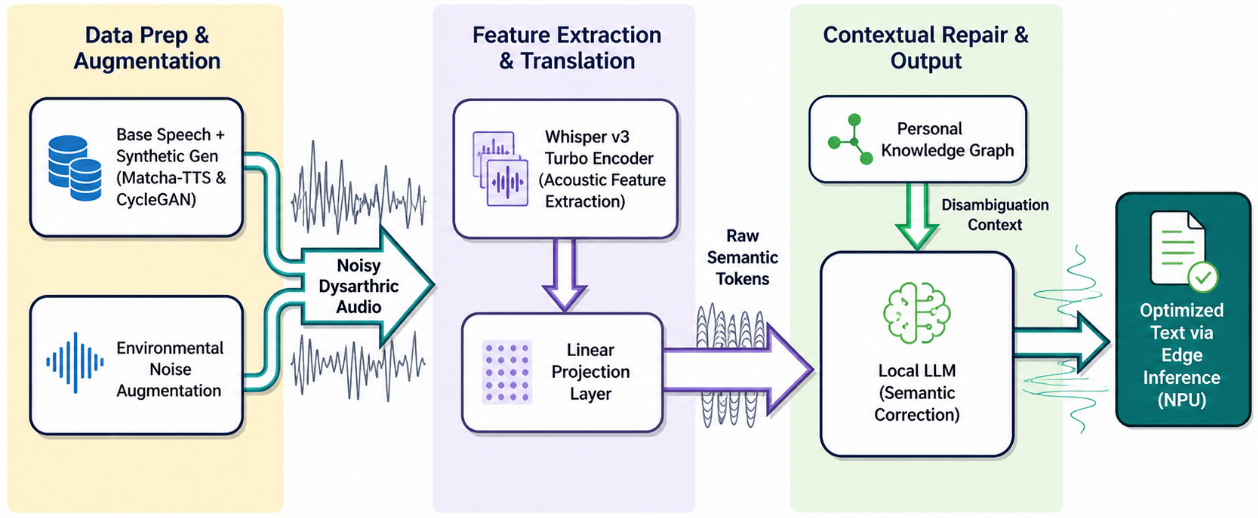
\includegraphics[width=1.0\textwidth]{Figures/system_pipeline_flow.png}
	\caption{Intelligent Fault Detection and Decision Pipeline}
	\label{fig:system_pipeline}
\end{figure}

\begin{figure}[H]
	\centering
	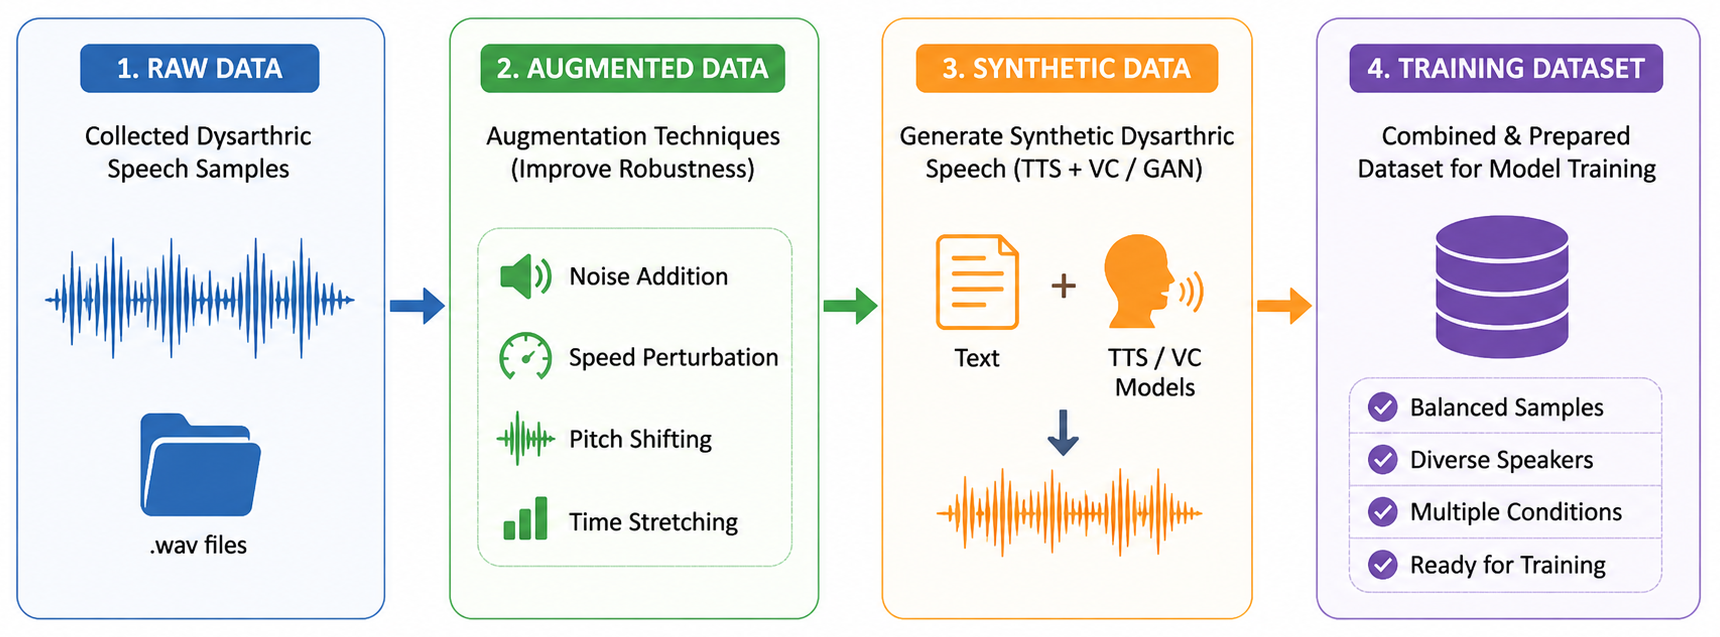
\includegraphics[width=1.0\textwidth]{Figures/data_pipeline_augmentation.png}
	\caption{Sensor Data Acquisition and Processing Pipeline}
	\label{fig:data_pipeline}
\end{figure}

\section{Experimental Techniques}

The system is developed and evaluated using:
\begin{itemize}
\item Real-time data acquisition from sensors under normal and fault conditions
\item Simulation of faults using controlled switching and variable loads
\item Training and testing of the Decision Tree model on labeled datasets
\item Evaluation of system latency and real-time performance
\item Validation of AI-generated insights and decision engine outputs
\item Comparison between traditional detection and intelligent system outputs
\end{itemize}

\section{Summary}

This chapter presented the design and architecture of the proposed intelligent fault detection and predictive governance system. It outlined the specifications, model selection, and methodology used to build a multi-layered pipeline combining embedded machine learning, decision intelligence, and generative AI. These design principles guide the implementation and evaluation discussed in the next chapter.